
\section{Introduction} % Bookmark information, displayed in the progress tree


\subsection{Motivation}
\begin{frame}[red] %hmm.. thought i could change colour here :S
\frametitle{Motivation} 
\begin{columns}
  \begin{column}{0.5\textwidth}
    \begin{itemize} \vspace{-1.5em}
      \item Many Shortest Path Queries
      \begin{itemize} 
      %http://techcrunch.com/2011/03/11/marissa-mayer-40-of-google-maps-usage-is-mobile-and-there-are-150-million-mobile-users/
      \gitem 40 \% of Google Maps usage is mobile %100 million users in August 2010
      %http://techcrunch.com/2011/05/25/google-maps-for-mobile-stats/
      \gitem 200+ million active mobile users as of may 2011
      %http://techcrunch.com/2011/03/11/marissa-mayer-40-of-google-maps-usage-is-mobile-and-there-are-150-million-mobile-users/
      \gitem Users drive 12 billion miles a year with Google Maps Navigation
      %http://blog.hubspot.com/blog/tabid/6307/bid/10829/5-Google-Local-Stats-Every-Marketer-Should-Know-Data.aspx
      \ritem 20 \% of Google searches are for local information 
      \end{itemize}
    \end{itemize}
  {
      \tiny \color{lightgray}
       http://techcrunch.com/2011/03/11/marissa-mayer-40-of-google-maps-usage-is-mobile-and-there-are-150-million-mobile-users/ \\
       http://techcrunch.com/2011/05/25/google-maps-for-mobile-stats/ \\
       http://blog.hubspot.com/blog/tabid/6307/bid/10829/5-Google-Local-Stats-Every-Marketer-Should-Know-Data.aspx \\
  }
  \end{column}
  \begin{column}[t]{0.5\textwidth}
  \vspace{-2em}
    \begin{figure}
    \includegraphics[width=0.70\textwidth]{images/mobilemaps} 
%     \caption{Google Maps Navigation}
    \end{figure}
  \end{column}
\end{columns}
\end{frame}

\begin{frame}[red] %hmm.. thought i could change colour here :S
\frametitle{Why is caching necessary}

$\bullet$ Shortest Path calculation is expensive

\begin{figure}[hbt]
  \center
  \scalebox{0.9} {
  \begin{tabular}{@{}c@{ }c@{ }c@{ }c@{}}\hline
   Source & Target & Travel & Response \\
          &    & time (s) & time (ms) \\
   \hline \hline
   Capitol Building & The Smithsonian & 372 & 101.24 \\\hline
   The Smithsonian & Washington, DC & 419 & 110.94 \\\hline
   White house & War Memorials & 41831 & 168.44 \\\hline
   White house & Capitol Building & 75805 & 278.44 \\\hline
   White house & Statue of Liberty & 88947 & 362.8 \\\hline
   Capitol Building & Mount Rushmore & 99456 & 364.68 \\\hline
   White house & Golden Gate Bridge & 108353 & 342.8 \\\hline
    \end{tabular}
    }\\
    \vspace{1em}Google Directions API
\end{figure}
\end{frame}




\subsection{Setting}
\begin{frame}[red] %hmm.. thought i could change colour here :S
\frametitle{Setting}
\begin{columns}
  \begin{column}{0.5\textwidth}
  Web search scenario: { \\ \tiny [Maarkatos et al., Computer Communications 2001]}
    \begin{itemize}
    \item Can have a cache at either a proxy or server site
    \item Saves response- or computation- time
    \item Cache stores web search results
    \item Existing cache algorithms include:\\ |{\it Least Recently Used} \\|{\it Highest Query Frequency}
    \end{itemize}
  \end{column}
  \begin{column}[t]{0.5\textwidth}
    \vspace{-2em}
    \begin{figure}
    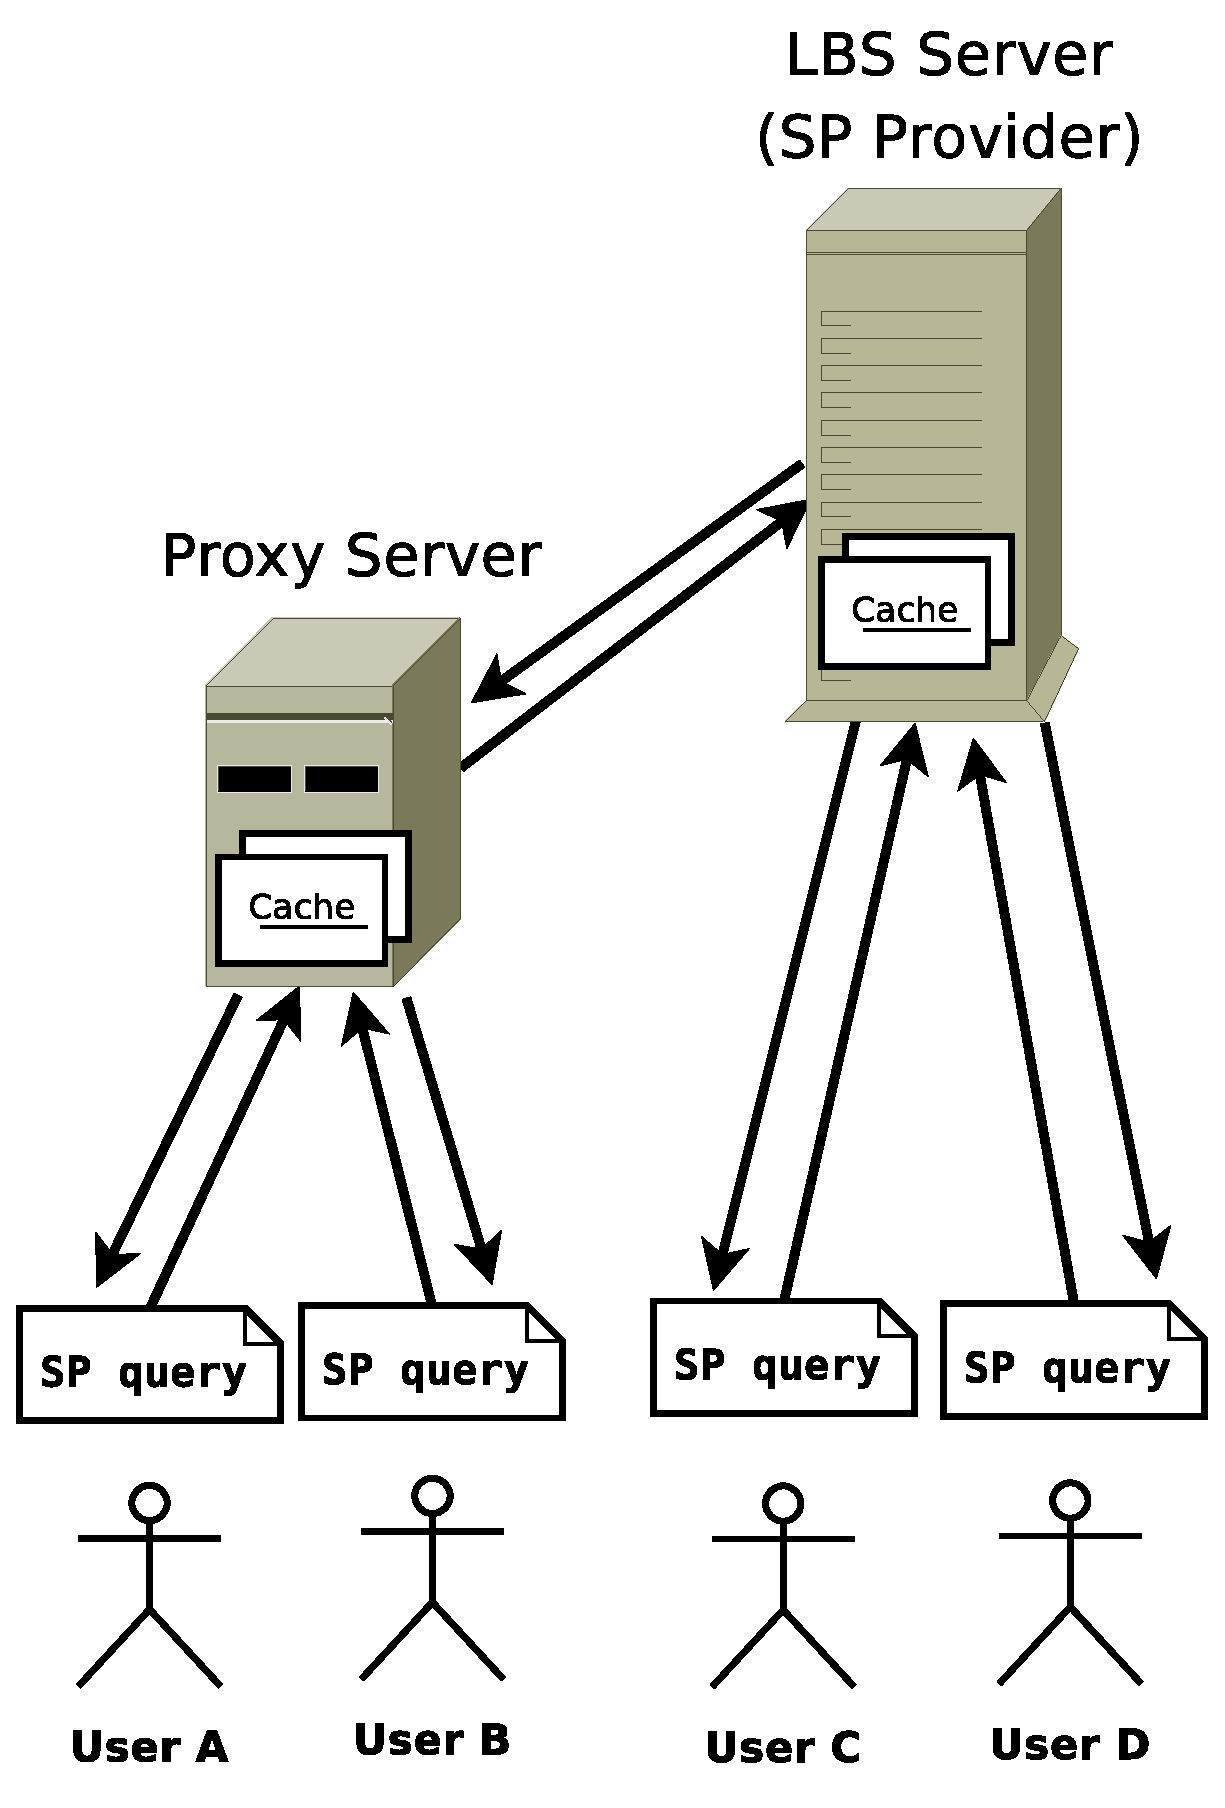
\includegraphics[width=1.05\textwidth]{images/scenario} 
    \caption{Web Search}
    \end{figure}
  \end{column}
\end{columns}
\end{frame}


\begin{frame}[red] %hmm.. thought i could change colour here :S
\frametitle{How does a Shortest Path Cache Work?} %Motivation
\begin{columns}
  \begin{column}{0.5\textwidth}
\vspace{-1.5em}

\begin{tabularx}{\textwidth}{|l|X|} \hline
\multicolumn{2}{|c|}{\bf Cache Content} \\\hline \hline
Path & Shortest Path \\\hline
1 & V1,V2,V3,V4,V7,V8,V9 \\\hline
2 & V1,V2,V3,V4,V5,V6 \\\hline
3 & V5,V4,V7 \\\hline
\end{tabularx}

\vspace{2em}

\begin{tabularx}{\textwidth}{|l|l|X|} \hline
\multicolumn{3}{|c|}{\bf Queries} \\\hline \hline
Query & Result & Path \\\hline
$Q_{V1,V9}$ & HIT & 1\\\hline
$Q_{V2,V5}$ & HIT & 2\\\hline
$Q_{V5,V9}$ & MISS & N/A\\\hline
\end{tabularx}


%   Existing Cache Problems: 
%     \begin{itemize}
%     \item Exact matching vs. partial matching
%     \item Cache structure does not support return of partial cache item
%     \item Different queries / paths require different processing cost %No cost model exist for shortest path
%     \end{itemize}
  \end{column}
  \begin{column}[t]{0.5\textwidth}
  \vspace{-2.7em}
    \begin{figure}
    \includegraphics[width=1\textwidth]{images/mobilemaps} 
%     \caption{Google Maps Navigation}
    \end{figure}  \end{column}
\end{columns}
\end{frame}


\subsection{Problem}
\begin{frame}[red] %hmm.. thought i could change colour here :S
\frametitle{How do we optimize the Cache Performance?}

  Benefit is expected cost saved:
    \begin{itemize}
    \item On server: computation time
    \item On proxy: communication time
    \end{itemize}

\vspace{1.5em}

We need to answer:
\begin{itemize}
%     \itemsep -2pt
    \item Which queries $Q_{s,t}$ can be answered by the path $P_{a,b}$?
    \item For query $Q_{s,t}$, what are the cost savings?
\end{itemize}

\vspace{1.5em}
  Given a: 
    \begin{itemize}
    \item Cache Size Budget 
    \item Query Log
    \end{itemize}
  Then build a cache $\Psi$ with max benefit $\gamma(\Psi)$\\
\end{frame}


\begin{frame}[color=red] %hmm.. thought i could change colour here :S
    \begin{figure}
    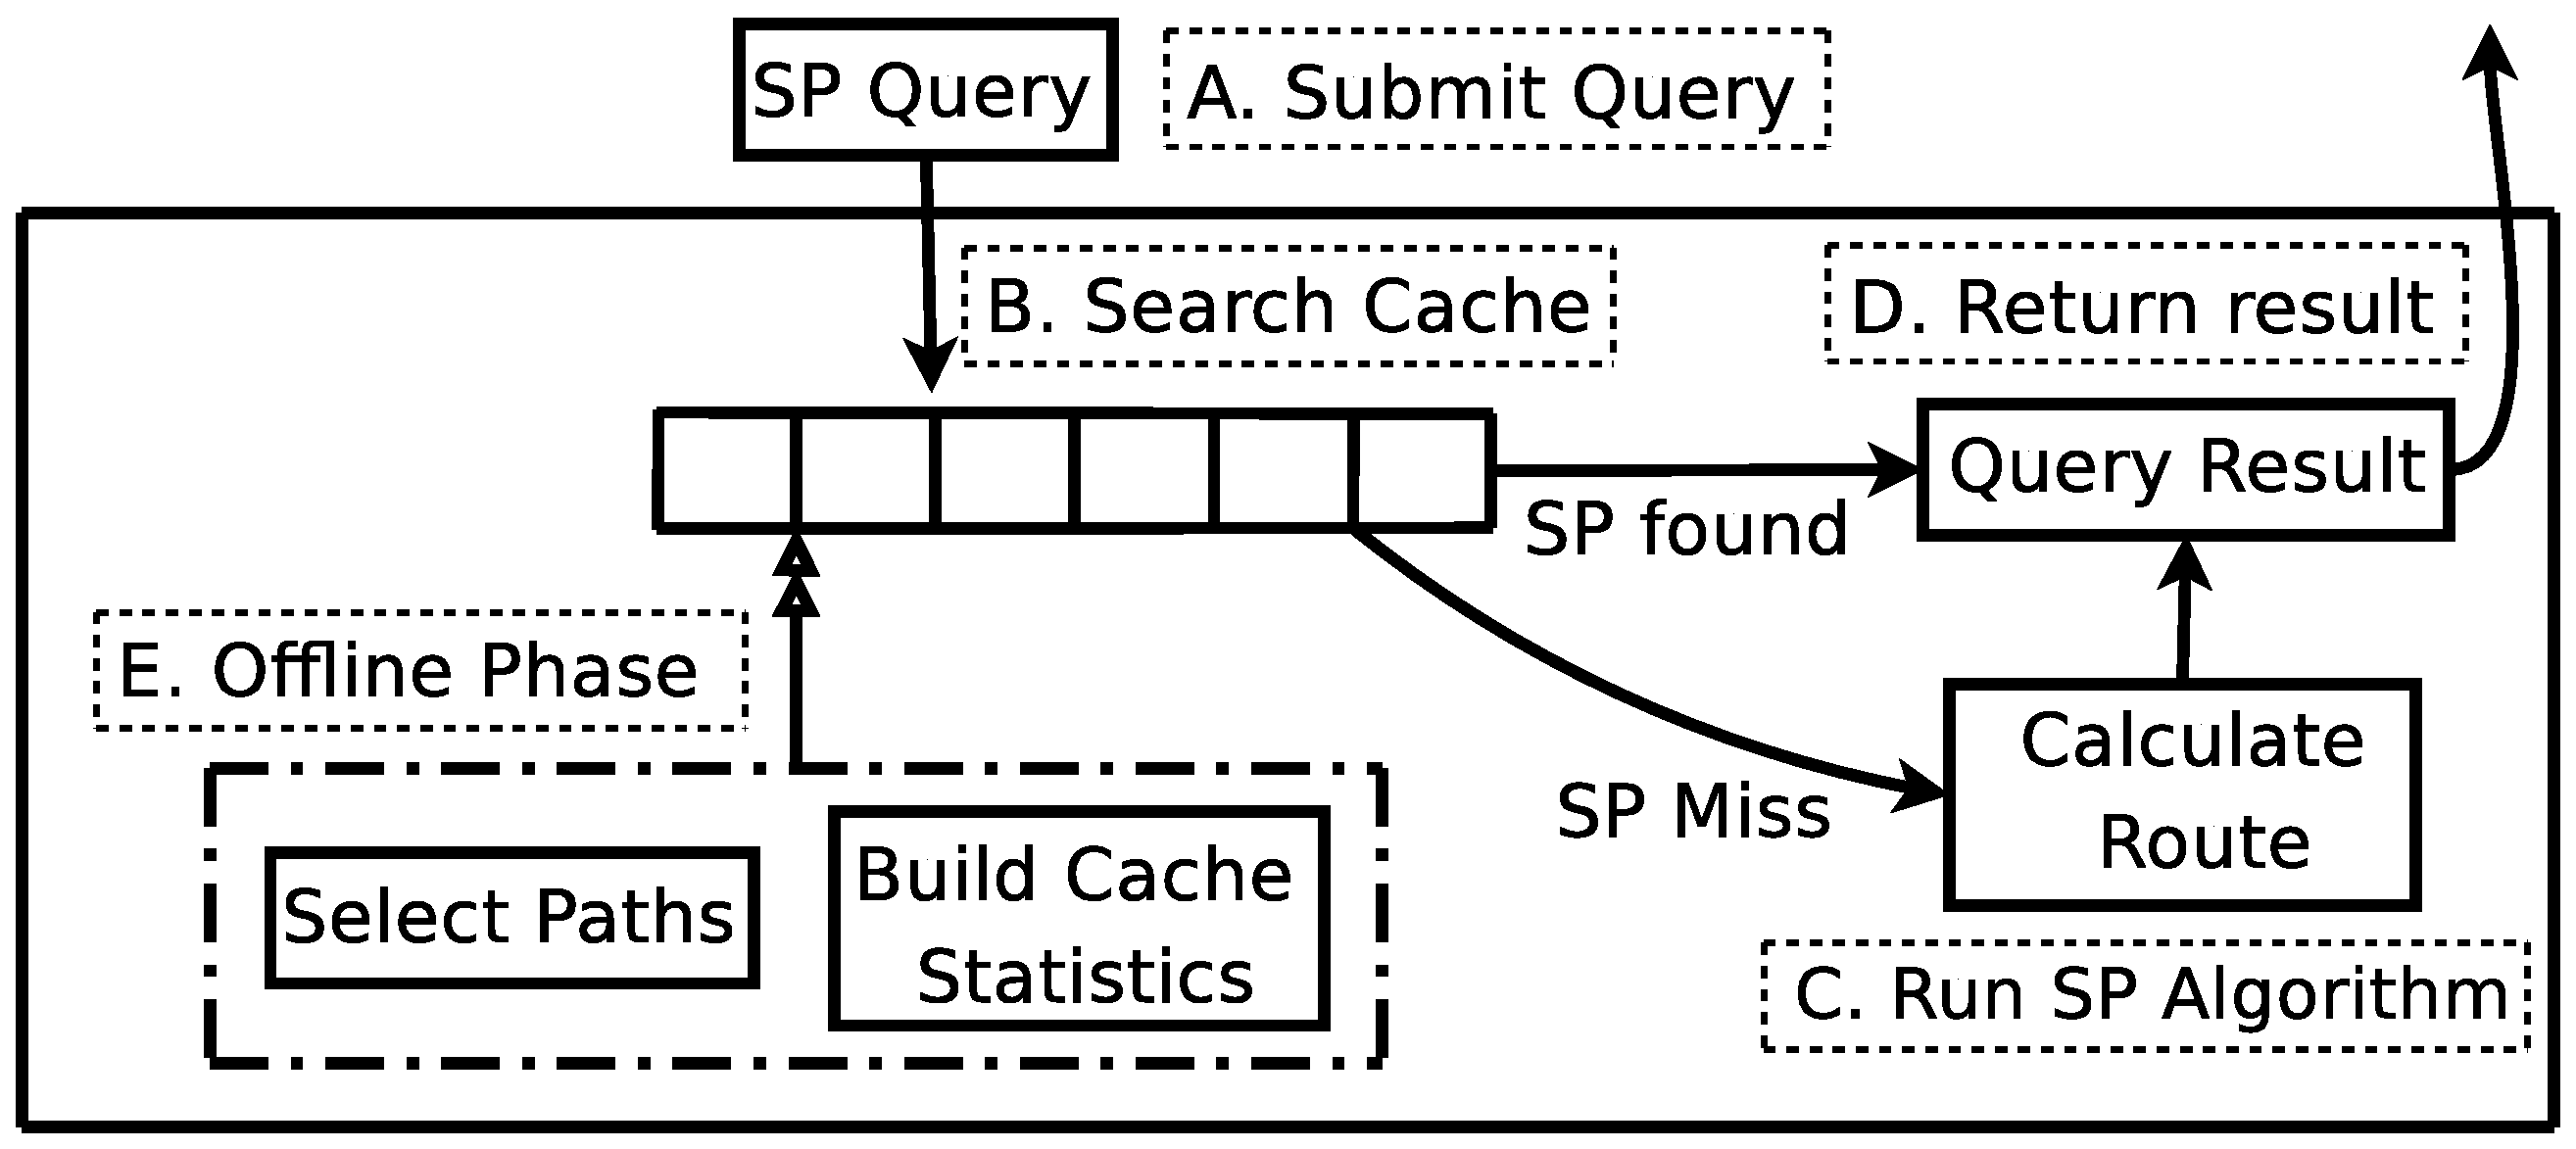
\includegraphics[width=1.05\textwidth]{images/routequery} 
    \
    \end{figure}

\begin{columns}
  \begin{column}{0.5\textwidth}
    \vspace{-0.8em}
    \begin{itemize}
    \itemsep -2pt
      \item Systematic model for benefit
      \item Techniques for query log statistics extraction 
    \end{itemize}
  \end{column}
  \begin{column}{0.6\textwidth}
    \vspace{-1.3em}
    \begin{itemize}
     \itemsep -2pt
      \item Efficient caching structure
      \item Shortest Path benchmarking techniques
    \end{itemize}
  \end{column}
\end{columns}
\end{frame}




